\cleardoublepage
\chapter{Metodolog�as}

Este proyecto ha seguido la filosof�a de las metodolog�as �giles, es decir, un desarrollo e incremental.\newline

Dado el car�cter din�mico de la disponibilidad del tiempo, se ha optado por una planificaci�n \textbf{Kanban}, una vez definidos los requisitos y plan de acci�n del proyecto.\newline

Adem�s ha sido vital afrontar la filosof�a DevOps, aplicando desde el comienzo del proyecto la integraci�n continua, para asegurar la salud del producto con cada nueva iteraci�n, ya que al trabajar directamente con la \acrshort{API} del demonio de Docker, cualquier m�nimo cambio afectaba al resto del proyecto.

\section{Extreme Programming}

Extreme Programming es una pr�ctica bastante extendida en el mundo del desarrollo de software. Obliga a definir la estructura del c�digo e incluso los tests antes de desarrollar el producto final, de tal manera, en primer lugar se dise�an y se implementan los tests, los cuales fallar�n hasta que la funcionalidad est� implementada completamente.\newline

Esta metodolog�a obliga al programador a pensar en el dise�o en un primer lugar, dotando al software de mas calidad.

\section{Kanban}

Kanban es un modelo �gil de organizaci�n del desarrollo de software que se caracteriza en la divisi�n de las tareas en diferentes estados, t�picamente, \textit{PENDIENTE}, \textit{EN PROGRESO} y \textit{TERMINADO}. \newline

Se ha utilizado la gesti�n de proyectos en el propio repositorio que ofrece la plataforma GitHub\footnote{https://github.com/mtenrero/ATQ-Director/projects/1} para que estuviese disponible para la comunidad de forma sencilla. Adem�s ofrece sincronizaci�n autom�tica de tareas basada en \textit{Issues} y \textit{Pull Requests}.\newline


\begin{figure}[h]
    \centering
    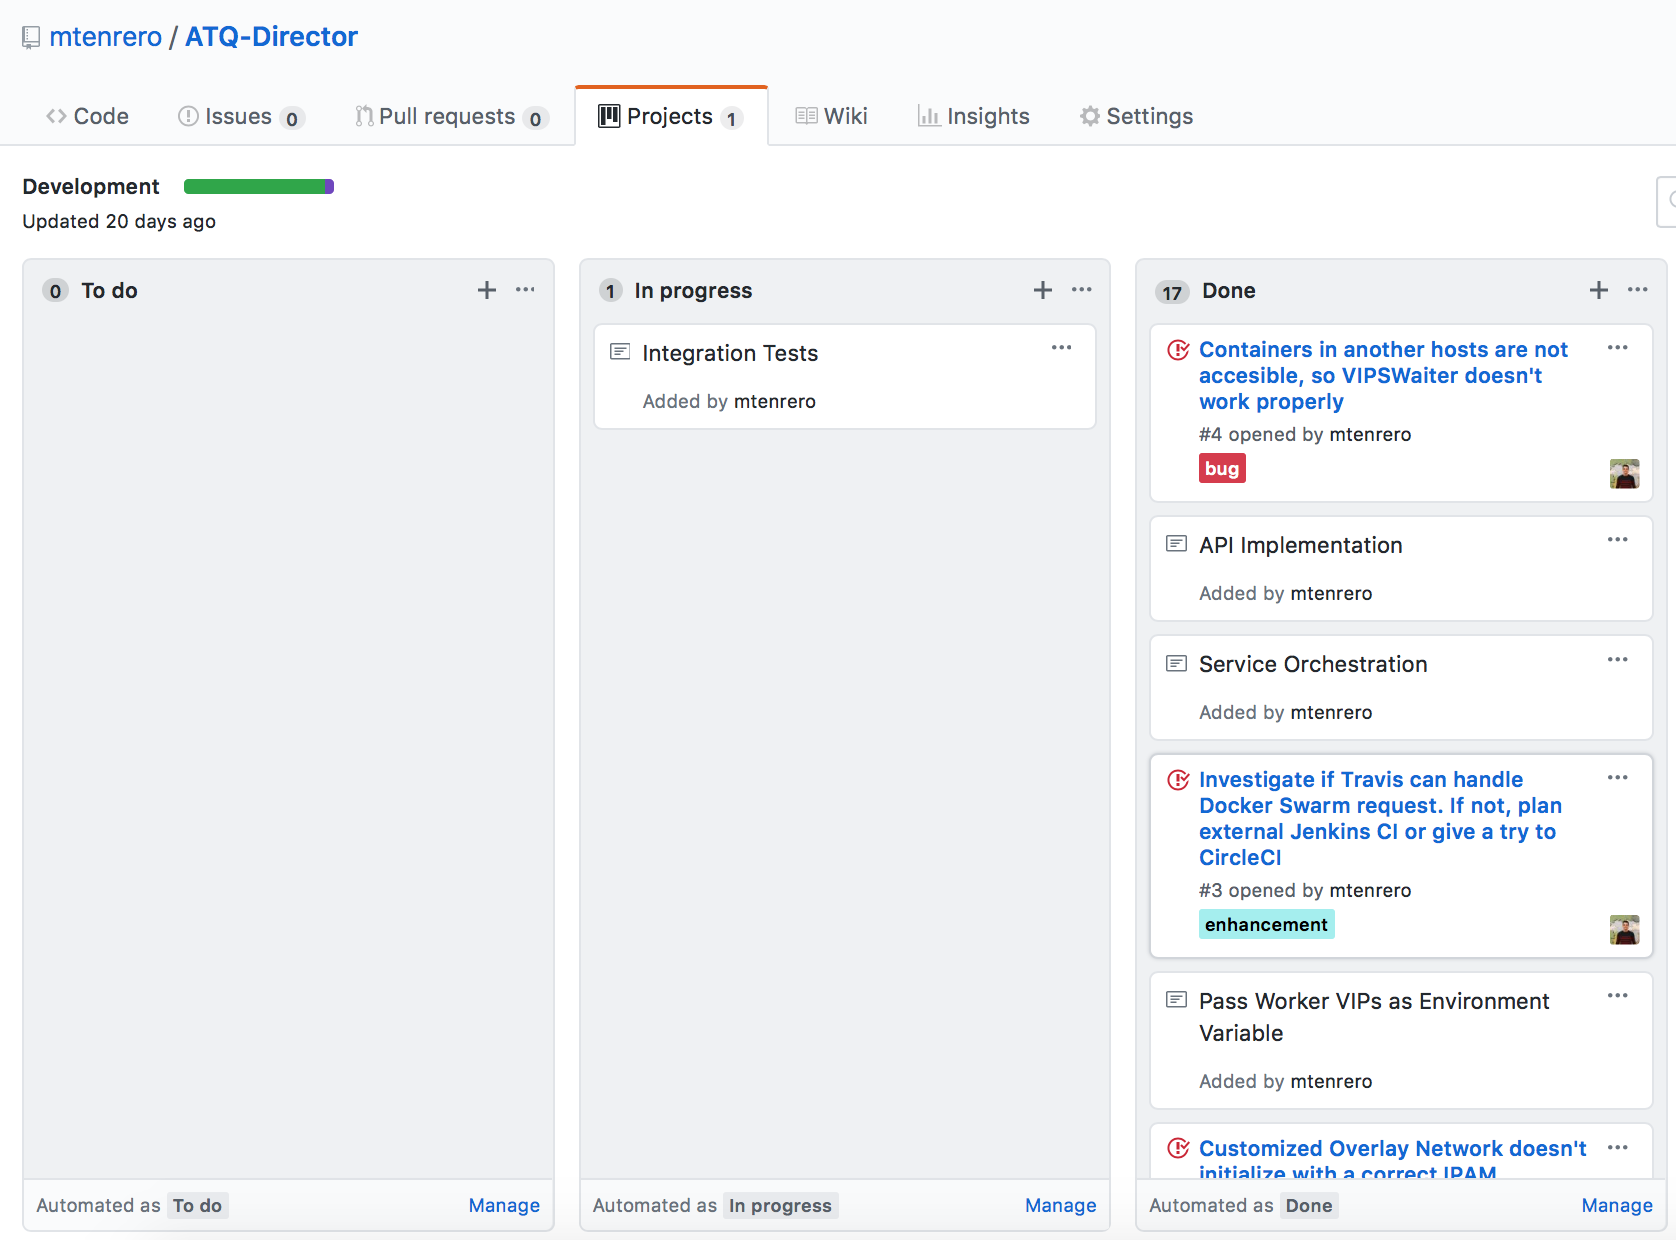
\includegraphics[width=1\textwidth]{kanban-github}
    \caption{Tablero Kanban del proyecto en GitHub}
    \label{fig:kanban}
\end{figure}